\documentclass{article}

\usepackage{math}
\usepackage{xcolor}

% GRAPHICS 
\usepackage{graphicx}

\colorlet{lightblue}{blue!50!cyan}

% TIKZ
\usepackage{tikz,pgfplots}
\pgfplotsset{compat=1.15}
\usepgfplotslibrary{fillbetween}
\usetikzlibrary{external}
\usepgfplotslibrary{external}
\tikzexternalize[prefix=optimization/]
\pgfplotsset{generalPlotOptions/.style={%
  width=4cm,
  height=4cm,
  xmin=-1,xmax=1,
  axis lines=center,
  axis line style={thick,latex-latex},
  xlabel={$x$},
  label style={font=\footnotesize},
  x label style={at={(axis cs:1.13,0)},anchor=north east},
  ticks=none,
  xticklabel=\empty,
  yticklabel=\empty,
  samples=501,
  clip mode=individual,
  no markers,
  % solid,
  every axis plot/.append style={thick}}}

\pgfplotsset{gradientPlotOptions/.style={%
  ymin=-1,ymax=1,
  ylabel={$\nabla\! f(x)$},
  y label style={at={(axis cs:0,1.13)},anchor=north east}}}

\pgfplotsset{functionPlotOptions/.style={%
  ymin=-0.2,ymax=1.8,
  ylabel={$f(x)$},
  y label style={at={(axis cs:0,1.93)},anchor=north east}}}
  
\newcommand{\gradientPlotSetup}{%
  \addplot [name path=m,lightblue] {0.2*x};
  \addplot [name path=L,lightblue] {2*x};
  \addplot [fill=gray!20] fill between [of=m and L];
  %\draw (-1.1,-1.1) rectangle (1.1,1.1);
  }

\newcommand{\functionPlotSetup}{%
  \addplot [name path=m,lightblue] {0.4*x^2};  % 0.1*x^2  (scale by 4)
  \addplot [name path=L,lightblue] {4*x^2};    % x^2
  \addplot [fill=gray!20] fill between [of=m and L];
  \draw (-1.1,-0.3) rectangle (1.1,1.9);}

%%%%%%%%%%%%%%%%%%%%%%%%%%%%%%%%%%%%%%%%%%%%%%%%%%%%%%%%%%%%%%%%%%%%%%%%%%%%%%%%
\begin{document}

\tikzsetnextfilename{gradient_linear}
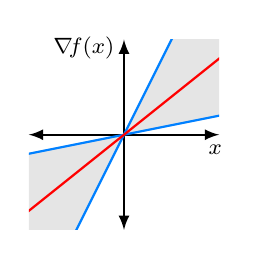
\begin{tikzpicture}
  \begin{axis}[generalPlotOptions,gradientPlotOptions]
    \gradientPlotSetup
    \addplot [red] {0.8*x};
  \end{axis}
\end{tikzpicture}

\tikzsetnextfilename{gradient_slope_restricted}
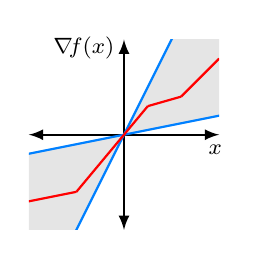
\begin{tikzpicture}
  \begin{axis}[generalPlotOptions,gradientPlotOptions]
    \gradientPlotSetup
    \addplot [red,domain=-1.00:-0.50] {0.2*x - 0.5};
    \addplot [red,domain=-0.50: 0.25] {1.2*x};
    \addplot [red,domain= 0.25: 0.60] {2*x/7 + 8/35};
    \addplot [red,domain= 0.60: 1.00] {x - 0.2};
  \end{axis}
\end{tikzpicture}

\tikzsetnextfilename{gradient_sector_bounded}
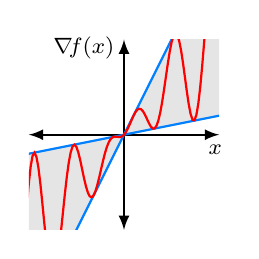
\begin{tikzpicture}
  \begin{axis}[generalPlotOptions,gradientPlotOptions]
    \gradientPlotSetup
    \addplot [red] {0.2*x + 1.8*x*(1-cos(15*deg(x)+90))/2};
  \end{axis}
\end{tikzpicture}

\tikzsetnextfilename{function_quadratic}
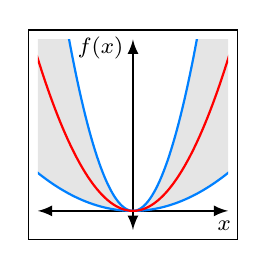
\begin{tikzpicture}
  \begin{axis}[generalPlotOptions,functionPlotOptions]
    \functionPlotSetup
    \addplot [red] {1.6*x^2};
  \end{axis}
\end{tikzpicture}

\tikzsetnextfilename{function_convex}
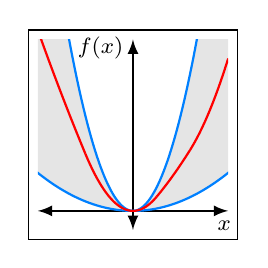
\begin{tikzpicture}
  \begin{axis}[generalPlotOptions,functionPlotOptions]
    \functionPlotSetup
    \addplot [red,domain=-1.00:-0.50] {4*x*(x-5)/10 - 0.5};
    \addplot [red,domain=-0.50: 0.25] {4*3*x^2/5};
    \addplot [red,domain= 0.25: 0.60] {4*x*(5*x+8)/35 - 4/35};
    \addplot [red,domain= 0.60: 1.00] {4*x*(5*x-2)/10 + 2/5};
  \end{axis}
\end{tikzpicture}

\tikzsetnextfilename{function_quasiconvex}
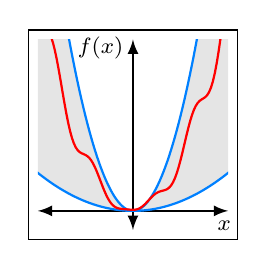
\begin{tikzpicture}
  \begin{axis}[generalPlotOptions,functionPlotOptions]
    \functionPlotSetup
    \addplot [red] {4*((11*x^2)/20 - (3*x*sin(15*deg(x) + 90))/50 - cos(15*deg(x) + 90)/250 + sqrt(2)/500)};
  \end{axis}
\end{tikzpicture}

\end{document}
